\part{Lecture 11: Eligibility Traces}
\title[RL Lecture 11]{Lecture 11: Eligibility Traces}  
\date{}  
\frame{\titlepage} 

%%%%%%%%%%%%%%%%%%%%%%%%%%%%%%%%%%%%%%%%%%%%%%%%%%%%%%%%%%%%%
%% Preface %%
%%%%%%%%%%%%%%%%%%%%%%%%%%%%%%%%%%%%%%%%%%%%%%%%%%%%%%%%%%%%%
\frame{\frametitle{Preface}
\begin{itemize}
	\item Recall $n$-step bootstrapping updates:
	\begin{equation*}
	\begin{split}
		g_{k:k+n} &= r_{k+1}+\gamma r_{k+2}+\cdots+\gamma^{n-1} r_{k+n}+\gamma^{n} \hat{v}_{k+n-1}(\bm{x}_{k+n}),\\
		g_{k:k+n} &= r_{k+1}+\gamma r_{k+2}+\cdots+\gamma^{n-1} r_{k+n}+\gamma^{n} \hat{q}_{k+n-1}(\bm{x}_{k+n}, u_{k+n}) .
	\end{split}
	\end{equation*}\pause
	\item Motivation: retrieve bootstrapped estimates between one-step updates and Monte Carlo.
	\begin{itemize}
		\item Use $n$ as degree of freedom to find the learning optimum.
	\end{itemize}\pause
	\item However, there are two significant drawbacks of $n$-step bootstrapping:
	\vspace{-0.4cm}
	\begin{itemize}
		\item Delay: we are looking $n$-steps into the future and, therefore, have to wait $n$-steps before we can perform the update.
		\item Memory: we have to store $n$ transitions until we can process them.
	\end{itemize}
\end{itemize}\pause
\begin{block}{Goal of today's lecture}
\begin{itemize}
	\item Find an algorithm with the same flexibility as $n$-step bootstrapping.
	\item Avoid the $n$-step disadvantages (delay, memory demand).
\end{itemize}
\end{block}
}

%%%%%%%%%%%%%%%%%%%%%%%%%%%%%%%%%%%%%%%%%%%%%%%%%%%%%%%%%%%%%%%%%%
\section{\texorpdfstring{$\lambda$}{Lambda}-Returns} 
%%%%%%%%%%%%%%%%%%%%%%%%%%%%%%%%%%%%%%%%%%%%%%%%%%%%%%%%%%%%%%%%%%
\begin{frame}
\frametitle{Table of Contents}
\tableofcontents
\end{frame}

%%%%%%%%%%%%%%%%%%%%%%%%%%%%%%%%%%%%%%%%%%%%%%%%%%%%%%%%%%%%%
%% General Averiging of $n$-Step Returns %%
%%%%%%%%%%%%%%%%%%%%%%%%%%%%%%%%%%%%%%%%%%%%%%%%%%%%%%%%%%%%%
\frame{\frametitle{General Averaging of $n$-Step Returns}
\begin{columns}[t,onlytextwidth]
\begin{column}{0.35\textwidth}
\begin{minipage}[c]{\linewidth}
\begin{figure}
	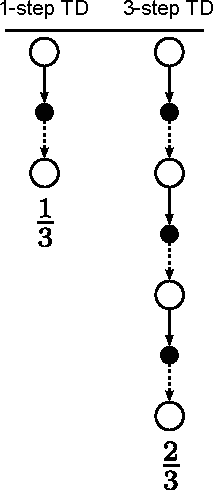
\includegraphics[width=2.5cm]{fig/lec11/Average_Bootstrap_Example.pdf}
	\caption{Exemplary averaging of $n$-step retuns}
	\label{fig:Average_Bootstrap_Example}
\end{figure}
\end{minipage}
\end{column}
\hfill
\begin{column}{0.6\textwidth}
\begin{minipage}[c]{\linewidth}
\begin{itemize}
	\item Averaging different $n$-step returns is possible without introducing a bias (if sum of weights is one).
	\item Example on the left:
	\begin{equation*}
		g = \frac{1}{3}g_{k:k+1} + \frac{2}{3}g_{k:k+3}
	\end{equation*}
	\item Horizontal line in backup diagram indicates the averaging.\pause 
	\item Enables additional degree of freedom to reduce prediction error. \pause
	\item Such updates are called \hl{compound updates}.
\end{itemize}
\end{minipage}
\end{column}
\end{columns}
}

%%%%%%%%%%%%%%%%%%%%%%%%%%%%%%%%%%%%%%%%%%%%%%%%%%%%%%%%%%%%%
%% $\lambda$-Return (1) %%
%%%%%%%%%%%%%%%%%%%%%%%%%%%%%%%%%%%%%%%%%%%%%%%%%%%%%%%%%%%%%
\frame{\frametitle{$\lambda$-Return (1)}
\begin{columns}[t,onlytextwidth]
\begin{column}{0.45\textwidth}
\begin{minipage}[c]{\linewidth}
\begin{figure}
	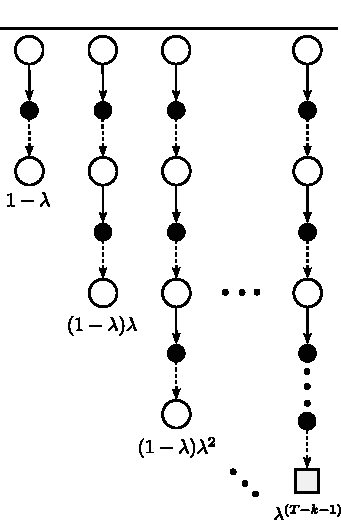
\includegraphics[width=4.2cm]{fig/lec11/Lambda_Return_Backup.pdf}
	\caption{Backup diagram for $\lambda$-returns}
	\label{fig:Lambda_Return_Backup}
\end{figure}
\end{minipage}
\end{column}
\hfill
\begin{column}{0.55\textwidth}
\begin{minipage}[c]{\linewidth}
\begin{itemize}
	\item \hl{$\lambda$-return}: is a compound update with exponentially decaying weights:
	\begin{equation}
		g_k^\lambda = (1-\lambda)\sum_{n=1}^{\infty}\lambda^{(n-1)}g_{k:k+n}\,.
		\label{eq:lambda_return}
	\end{equation}
	\item Parameter is $\lambda\in\left\{\mathbb{R}|0\leq \lambda \leq 1\right\}$.
	\item Geometric series of weights is one:
	\begin{equation*}
		(1-\lambda)\sum_{n=1}^{\infty}\lambda^{(n-1)} = 1
	\end{equation*}
\end{itemize}
\end{minipage}
\end{column}
\end{columns}
}

%%%%%%%%%%%%%%%%%%%%%%%%%%%%%%%%%%%%%%%%%%%%%%%%%%%%%%%%%%%%%
%% $\lambda$-Return (2) %%
%%%%%%%%%%%%%%%%%%%%%%%%%%%%%%%%%%%%%%%%%%%%%%%%%%%%%%%%%%%%%
\frame{\frametitle{$\lambda$-Return (2)}
\onslide<1->{\begin{itemize}
	\item Rewrite $\lambda$-return for episodic tasks with termination at $k=T$:
		\begin{equation}
		g_k^\lambda = (1-\lambda)\sum_{n=1}^{T-k-1}\lambda^{(n-1)}g_{k:k+n} + \lambda^{T-k-1}g_k\,.
		\label{eq:lambda_return_episodic}
	\end{equation}
	\item Return $g_k$ after termination is weighted with residual weight $\lambda^{T-k-1}$.}
	\onslide<2->{\item Above, \eqref{eq:lambda_return_episodic} includes two special cases:
	\begin{itemize}
		\item If $\lambda=0$: becomes TD(0) update.
		\item If $\lambda=1$: becomes MC update.
	\end{itemize}}
\end{itemize}
\onslide<1->{\begin{figure}
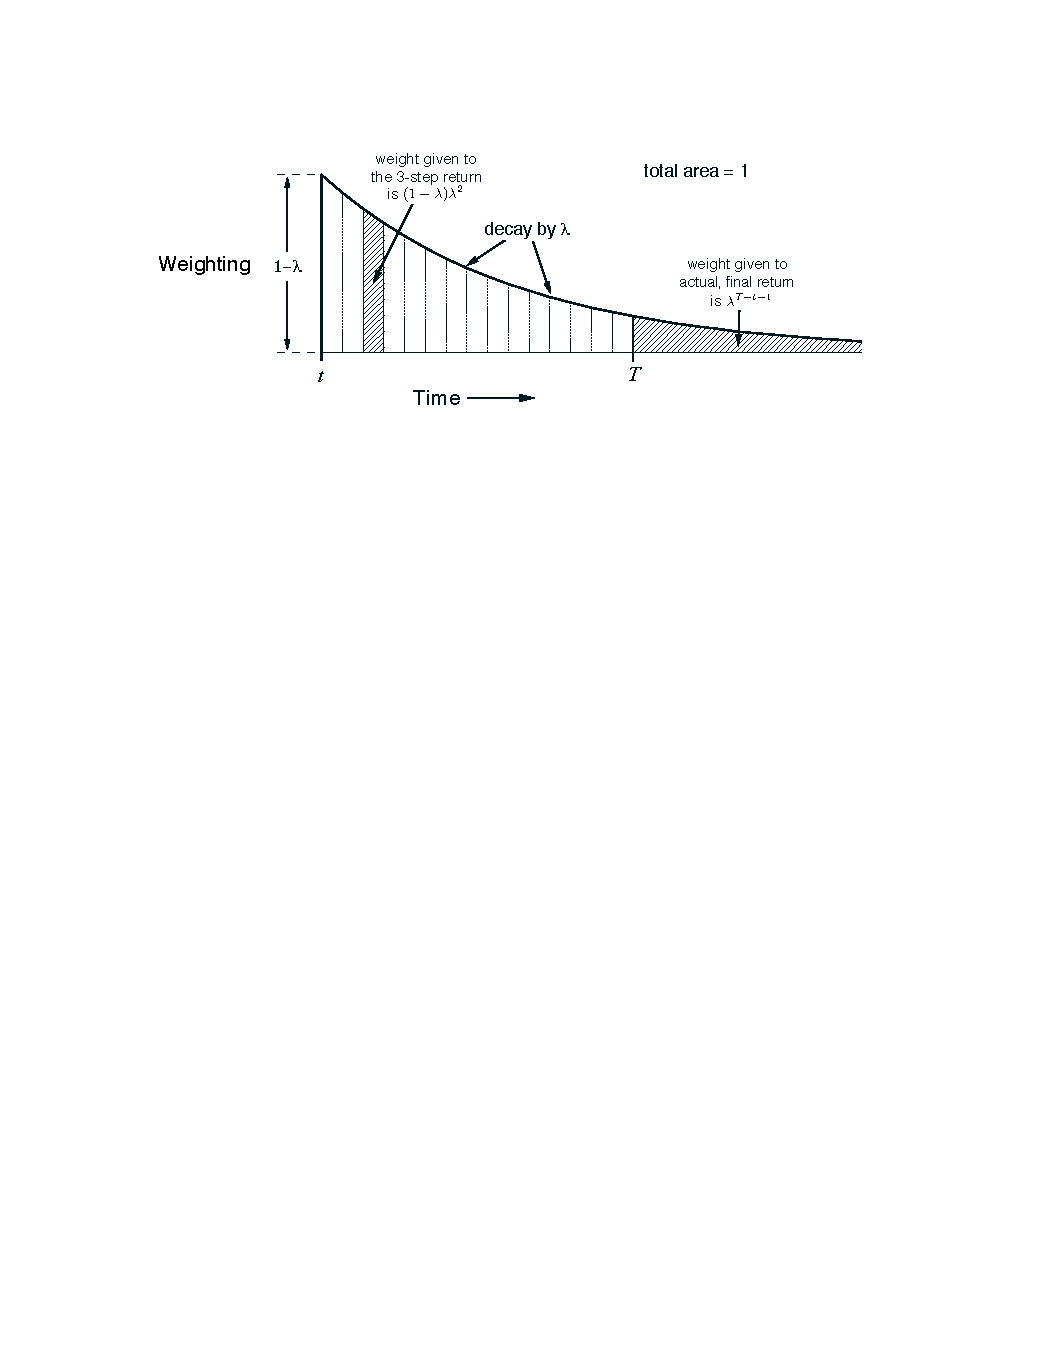
\includegraphics[height=3cm]{fig/lec11/Lambda_Weighting_Series.pdf}
\caption{Weighting overview in $\lambda$-return series (source: R. Sutton and G. Barto, Reinforcement learning: an introduction, 2018, \href{https://creativecommons.org/licenses/by-nc-nd/2.0/}{CC BY-NC-ND 2.0})}
\label{fig:Lambda_Weighting_Series}
\end{figure}}
}

%%%%%%%%%%%%%%%%%%%%%%%%%%%%%%%%%%%%%%%%%%%%%%%%%%%%%%%%%%%%%
%% Offline $\lambda$-Return Semi-Gradient Algorithm %%
%%%%%%%%%%%%%%%%%%%%%%%%%%%%%%%%%%%%%%%%%%%%%%%%%%%%%%%%%%%%%
\frame{\frametitle{Offline $\lambda$-Return Semi-Gradient Algorithm}
\begin{itemize}
	\item Applying semi-gradient updates with fct. approximation we receive:
		\begin{equation}
		\bm{w}_{k+1} = \bm{w}_k+\alpha\left[g_k^\lambda - \hat{v}(\bm{x}_k, \bm{w}_k)\right]\nabla_{\bm{w}}\hat{v}(\bm{x}_k, \bm{w}_k) .
		\label{eq:lambda_return_offline_updates}
	\end{equation}\pause\vspace{-0.25cm}
	\item Offline refers to that $\bm{w}$ is not changed until the episode's end.
\end{itemize}\pause
\begin{figure}
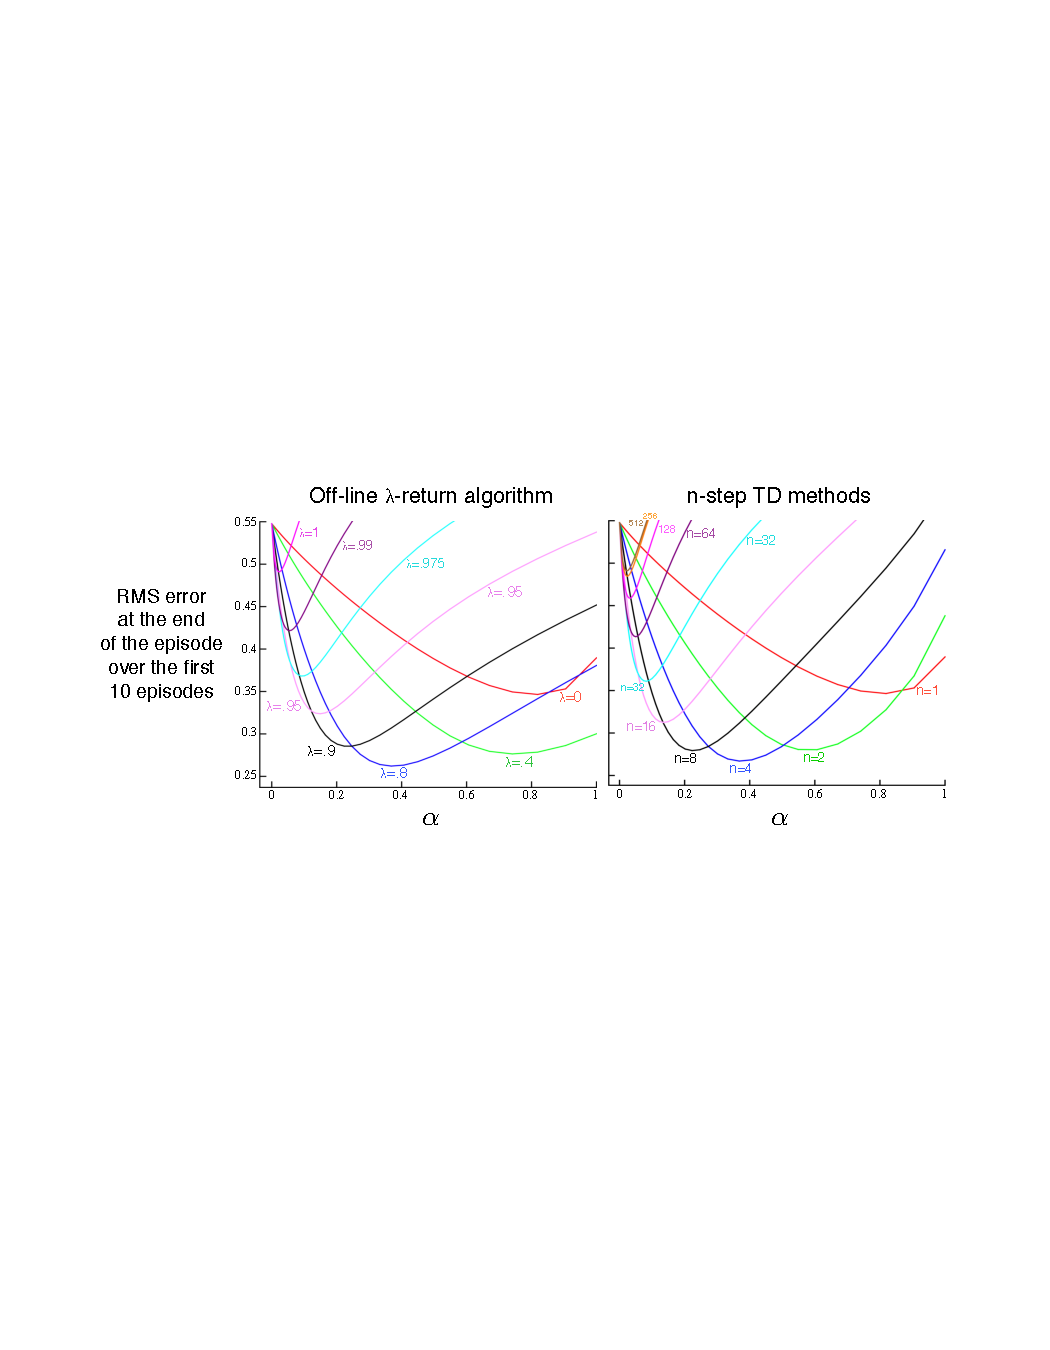
\includegraphics[height=4.3cm]{fig/lec11/Offline_Lamba_vs_n_step_TD.pdf}
\caption{Prediction accuracy comparison based on 19-state random walk example from \figref{fig:Random_Walk_19_States} (source: R. Sutton and G. Barto, Reinforcement learning: an introduction, 2018, \href{https://creativecommons.org/licenses/by-nc-nd/2.0/}{CC BY-NC-ND 2.0})}
\label{fig:Offline_Lamba_vs_n_step_TD}
\end{figure}
}


%%%%%%%%%%%%%%%%%%%%%%%%%%%%%%%%%%%%%%%%%%%%%%%%%%%%%%%%%%%%%
%% Truncated $\lambda$-Returns %%
%%%%%%%%%%%%%%%%%%%%%%%%%%%%%%%%%%%%%%%%%%%%%%%%%%%%%%%%%%%%%
\frame{\frametitle{Truncated $\lambda$-Returns }
\begin{itemize}
	\item Using $\lambda$-returns as in \eqref{eq:lambda_return} is not feasible for continuing tasks.
	\item One would have to wait infinitely long to receive the trajectory.\pause
	\item Intuitive approximation: truncate $\lambda$-return after $h$ steps 
	\begin{equation}
		g_{k:h}^\lambda = (1-\lambda)\sum_{n=1}^{h-k-1}\lambda^{(n-1)}g_{k:k+n} + \lambda^{h-k-1}g_{k:h}\,.
		\label{eq:lambda_return_trunc}
	\end{equation}
	\item Horizon $h$ divides continuing tasks in rolling episodes.\pause
	\item The truncated $\lambda$-return \eqref{eq:lambda_return_trunc} can be used analogously to $n$-step returns in semi-gradient TD updates (cf. \algoref{algo:Semi_gradient_TD_nstep}).
\end{itemize}
}

%%%%%%%%%%%%%%%%%%%%%%%%%%%%%%%%%%%%%%%%%%%%%%%%%%%%%%%%%%%%%
%% Forward View %%
%%%%%%%%%%%%%%%%%%%%%%%%%%%%%%%%%%%%%%%%%%%%%%%%%%%%%%%%%%%%%
\frame{\frametitle{Forward View}
\onslide<1->{\begin{itemize}
	\item Both, $n$-step and $\lambda$-return updates, are based on a forward view.  
	\item We have to wait for future states and rewards to arrive before we are able to perform an update.}
	\onslide<2->{\item Currently, $\lambda$-returns are only an alternative to $n$-step updates with different weighting without a particular advantage.}
\end{itemize}
\onslide<1->{\begin{figure}
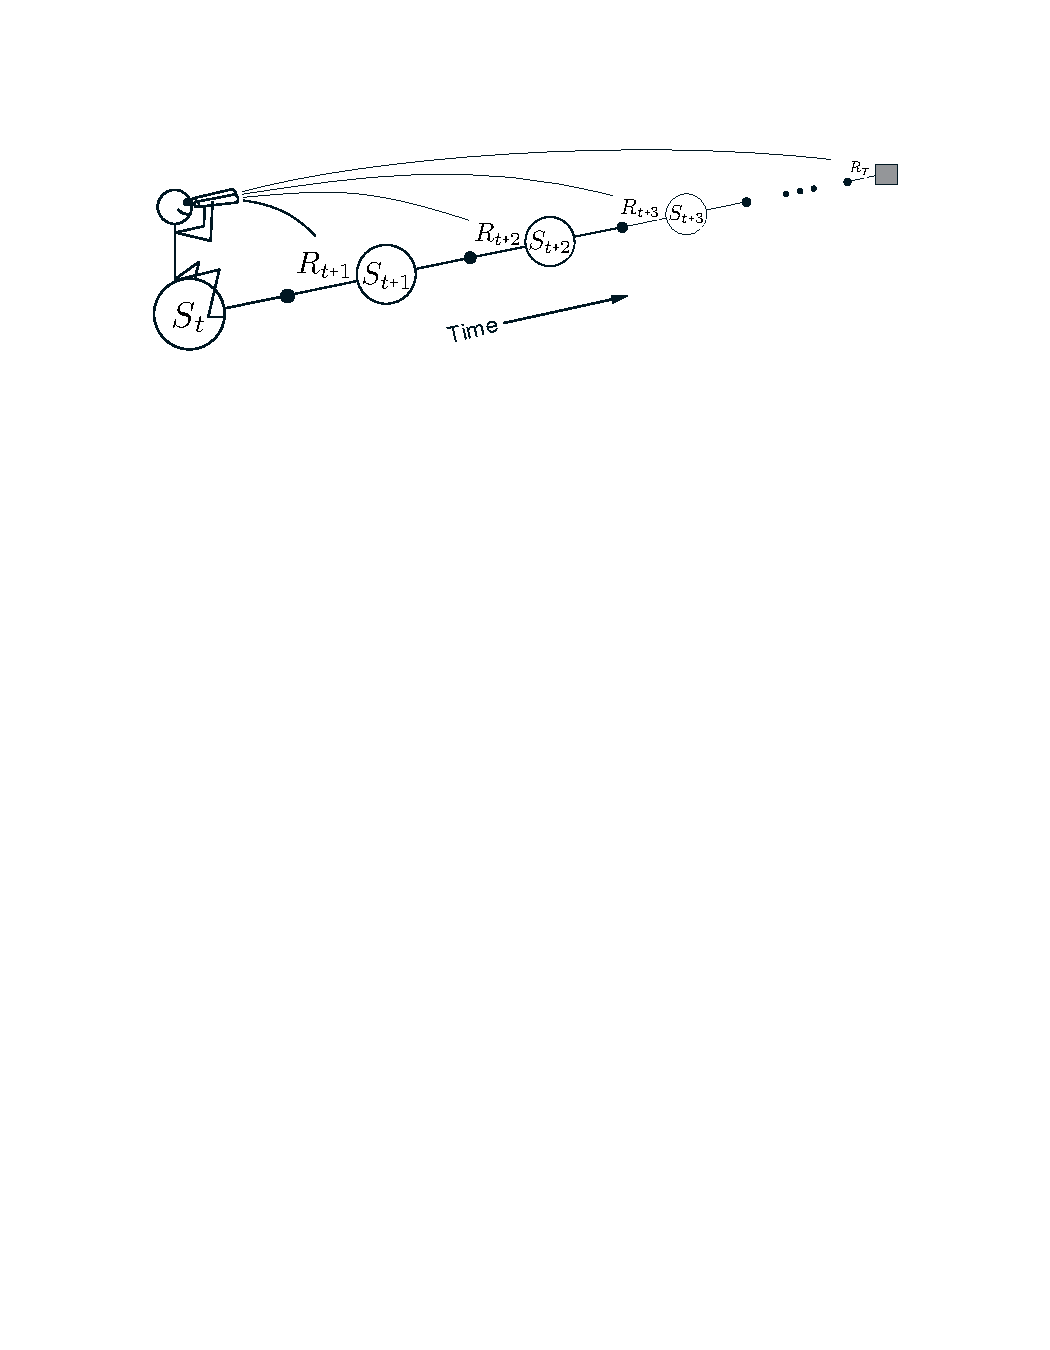
\includegraphics[height=2.5cm]{fig/lec11/Forward_View.pdf}
\caption{The forward view: an update of the current state value is evaluated by future transitions (source: R. Sutton and G. Barto, Reinforcement learning: an introduction, 2018, \href{https://creativecommons.org/licenses/by-nc-nd/2.0/}{CC BY-NC-ND 2.0})}
\label{fig:Forward_View}
\end{figure}}
}

%%%%%%%%%%%%%%%%%%%%%%%%%%%%%%%%%%%%%%%%%%%%%%%%%%%%%%%%%%%%%%%%%%
\section{TD(\texorpdfstring{$\lambda$}{Lambda})} 
%%%%%%%%%%%%%%%%%%%%%%%%%%%%%%%%%%%%%%%%%%%%%%%%%%%%%%%%%%%%%%%%%%
\begin{frame}
\frametitle{Table of Contents}
\tableofcontents[currentsection]
\end{frame}

%%%%%%%%%%%%%%%%%%%%%%%%%%%%%%%%%%%%%%%%%%%%%%%%%%%%%%%%%%%%%
%% Backward View %%
%%%%%%%%%%%%%%%%%%%%%%%%%%%%%%%%%%%%%%%%%%%%%%%%%%%%%%%%%%%%%
\frame{\frametitle{Backward View of TD($\lambda$)}
\onslide<1->{General idea:
\begin{itemize}
	\item Use $\lambda$-weighted returns looking into the past. 
	\item Implement this in a recursive fashion to save memory.}
	\onslide<2->{\item Therefore, an \hl{eligibility trace $\bm{z}_k$} denoting the importance of past events to the current state update is introduced. }
\end{itemize}
\onslide<1->{\begin{figure}
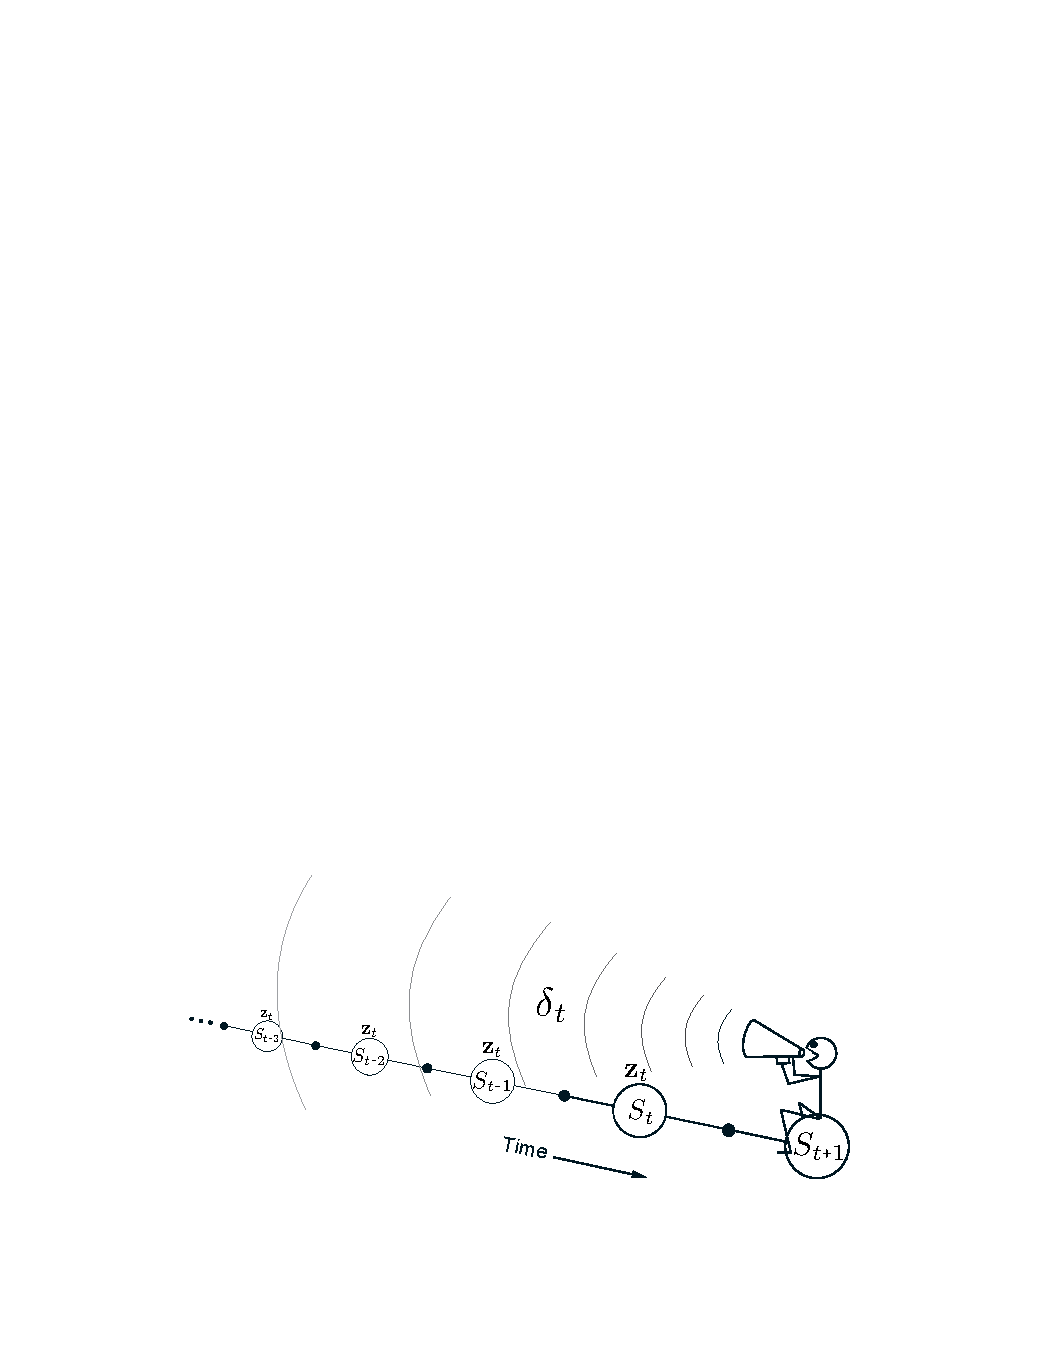
\includegraphics[height=3.5cm]{fig/lec11/Backward_View.pdf}
\caption{The backward view: an update of the current state value is evaluated based on a trace of past transitions (source: R. Sutton and G. Barto, Reinforcement learning: an introduction, 2018, \href{https://creativecommons.org/licenses/by-nc-nd/2.0/}{CC BY-NC-ND 2.0})}
\label{fig:Backward_View}
\end{figure}}
}

%%%%%%%%%%%%%%%%%%%%%%%%%%%%%%%%%%%%%%%%%%%%%%%%%%%%%%%%%%%%%
%% Eligibility Trace (1) %%
%%%%%%%%%%%%%%%%%%%%%%%%%%%%%%%%%%%%%%%%%%%%%%%%%%%%%%%%%%%%%
\frame{\frametitle{Eligibility Trace (1)}
Why is the exponential weighting particular suitable for TD($\lambda$)?\pause
\begin{itemize}
	\item Because we can easily implement this in a recursive fashion.\pause
\end{itemize}
\begin{block}{Exponential smoothing filter}
Let $x_k$ be an arbitrary signal sampled at equally distributed time steps $k$. Then, the filtered signal $y_k$ with an exponential window function of past observations is
\begin{equation}
	y_k = \beta x_k + (1-\beta)y_{k-1}, \quad k> 0 \quad \mbox{and} \quad y_0=x_0
	\label{eq:exp_smoothing_filter}
\end{equation}
with $\beta$ being the smoothing factor.  
\end{block}\pause
\begin{itemize}
	\item Above is a simple recursive exponential smoothing filter which converges for $k>>1$.
\end{itemize}
}

%%%%%%%%%%%%%%%%%%%%%%%%%%%%%%%%%%%%%%%%%%%%%%%%%%%%%%%%%%%%%
%% Eligibility Trace (2) %%
%%%%%%%%%%%%%%%%%%%%%%%%%%%%%%%%%%%%%%%%%%%%%%%%%%%%%%%%%%%%%
\frame{\frametitle{Eligibility Trace (2)}
With TD and function approximation 
\begin{itemize}
	\item the \hl{eligibility trace $z_k\in\mathbb{R}^\zeta$} is a vector with same dimensions as $\bm{w}$:
	\begin{equation}
\begin{split}
	\bm{z}_{0}&=0,\\
	\bm{z}_k &=\gamma\lambda\bm{z}_{k-1}+\nabla_{\bm{w}}\hat{v}(\bm{x}_k,\bm{w}_k).
\end{split}	
\label{eq:Elig_trace}
\end{equation}
	\item It tracks which components of $\bm{w}$ have contributed to recent state valuations. Here, \hl{$\lambda$} is also called the \hl{trace-decay parameter}.\pause
\end{itemize}
Further remarks:
\begin{itemize}
	\item $\bm{z}_k$ can be interpreted a short-term memory while $\bm{w}_k$ is the long-term memory within the learning process of $\hat{v}$.\pause
	\item Comparing \eqref{eq:Elig_trace} with the filter \eqref{eq:exp_smoothing_filter} it becomes obvious that $\bm{z}$ is not an idealized exp. filtered form of $\nabla_{\bm{w}}\hat{v}$.\pause
	\item Consider case $k\rightarrow\infty$ and $\nabla_{\bm{w}}\hat{v}(\bm{x}_k,\bm{w}_k)=\nabla_{\bm{w}}\hat{v}=\mbox{const.}$, then $\bm{z}$ is only a bias-free  trace of $\nabla_{\bm{w}}\hat{v}$ in the TD sense if $\lambda = 1$:
	\begin{equation*}
		 \bm{z}=\frac{\nabla_{\bm{w}}\hat{v}}{1-\gamma\lambda}.
	\end{equation*}
	\end{itemize}
}

%%%%%%%%%%%%%%%%%%%%%%%%%%%%%%%%%%%%%%%%%%%%%%%%%%%%%%%%%%%%%
%% Eligibility Trace (1) %%
%%%%%%%%%%%%%%%%%%%%%%%%%%%%%%%%%%%%%%%%%%%%%%%%%%%%%%%%%%%%%
\frame{\frametitle{Simplified Eligibility Trace Example}
\begin{itemize}
	\item Consider linear function approximation with a single state being the feature vector
		\begin{equation*}
			  \hat{v}(x_k, w) = x_k w \quad \rightarrow \quad \nabla_w \hat{v}(x_k, w) = x_k .
		\end{equation*}
	\item For illustration purpose we assume that $w$ is constant.
	\item Below is an example for the eligibility trace with $\lambda = 0.9, \gamma=1$.
\end{itemize}
	\begin{figure}
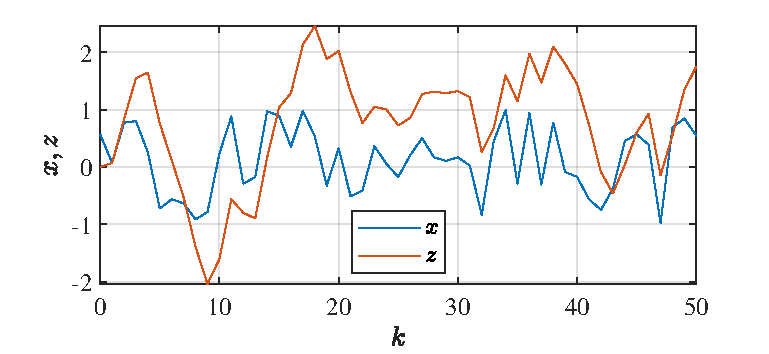
\includegraphics[height=4.0cm]{fig/lec11/Eglibility_Trace_Example.pdf}
\caption{Illustration of gradient $\nabla_w \hat{v}$ and corresponding trace $z$ based on \eqref{eq:Elig_trace} for single state example with linear function approximation}
\label{fig:Eglibility_Trace_Example}
\end{figure}	

}

%%%%%%%%%%%%%%%%%%%%%%%%%%%%%%%%%%%%%%%%%%%%%%%%%%%%%%%%%%%%%
%% Semi-Gradient TD($\lambda$) %%
%%%%%%%%%%%%%%%%%%%%%%%%%%%%%%%%%%%%%%%%%%%%%%%%%%%%%%%%%%%%%
\frame{\frametitle{Semi-Gradient TD($\lambda$)}
Together with \eqref{eq:Elig_trace} the semi-gradient TD($\lambda$) update is:
	\begin{equation}
\begin{split}
	\delta_k &=r_{k+1} + \gamma \hat{v}(\bm{x}_{k+1}, \bm{w}_k) -\hat{v}(\bm{x}_{k}, \bm{w}_k),\\
	 \bm{w}_{k+1} &=  \bm{w}_k + \alpha\delta_k\bm{z}_k .
\end{split}	
\label{eq:semi_grad_update_lambda_TD}
\end{equation}\pause
\vspace{-0.2cm}
\setlength{\algomargin}{0.5em}
\begin{algorithm}[H]
\small
\SetKwInput{Input}{input} 
\SetKwInput{Output}{output}
\SetKwInput{Init}{init}
\SetKwInput{Param}{parameter}
\Input{a policy $\pi$ to be evaluated}
\Input{a differentiable function $\hat{v}:\mathbb{R}^\kappa\times\mathbb{R}^\zeta\rightarrow\mathbb{R}$ with $\hat{v}(\bm{x}_T, \cdot)=0$}
\Param{step size $\alpha\in\left\{\mathbb{R}|0<\alpha<1\right\}$, decay rate $\lambda\in\left\{\mathbb{R}|0 \leq \lambda \leq 1\right\}$}
\Init{value-function weights $\bm{w}\in\mathbb{R}^\zeta$ arbitrarily}
 \For{$j=1,2,\ldots$ episodes}{
		initialize $\bm{x}_{0}$ and set $\bm{z}=0$\;
		\For{$k=0, 1, 2 \ldots $ time steps}{
			$u_k \leftarrow$ apply action from $\pi(\bm{x}_k)$\;
			observe $\bm{x}_{k+1}$ and $r_{k+1}$\;
			$\bm{z}\leftarrow \gamma\lambda\bm{z}+\nabla_{\bm{w}}\hat{v}(\bm{x}_k, \bm{w})$\;
			$\delta\leftarrow r_{k+1} +\gamma \hat{v}(\bm{x}_{k+1}, \bm{w}) - \hat{v}(\bm{x}_k, \bm{w})$\;
			$\bm{w} \leftarrow \bm{w} + \alpha\delta\bm{z}$\; 
			exit loop if $\bm{x}_{k+1}$ is terminal\;
		}
	}
\caption{Semi-gradient TD($\lambda$) (output: parameter vector $\bm{w}$ for $\hat{v}_\pi$)}
\label{algo:Semi_gradient_TD_lambda}
\end{algorithm}
}


%%%%%%%%%%%%%%%%%%%%%%%%%%%%%%%%%%%%%%%%%%%%%%%%%%%%%%%%%%%%%
%% Exemplary Comparison %%
%%%%%%%%%%%%%%%%%%%%%%%%%%%%%%%%%%%%%%%%%%%%%%%%%%%%%%%%%%%%%
\frame{\frametitle{Exemplary Comparison}
\begin{itemize}
	\item \hl{TD($\lambda$) is not an exact representation of offline $\lambda$-returns} (see below).
	\item For $\lambda=0$: matches exactly semi-gradient one-step TD ('TD(0)').
	\item For $\lambda=1$: mimics long-term Monte Carlo updates.   
\end{itemize}
\begin{figure}
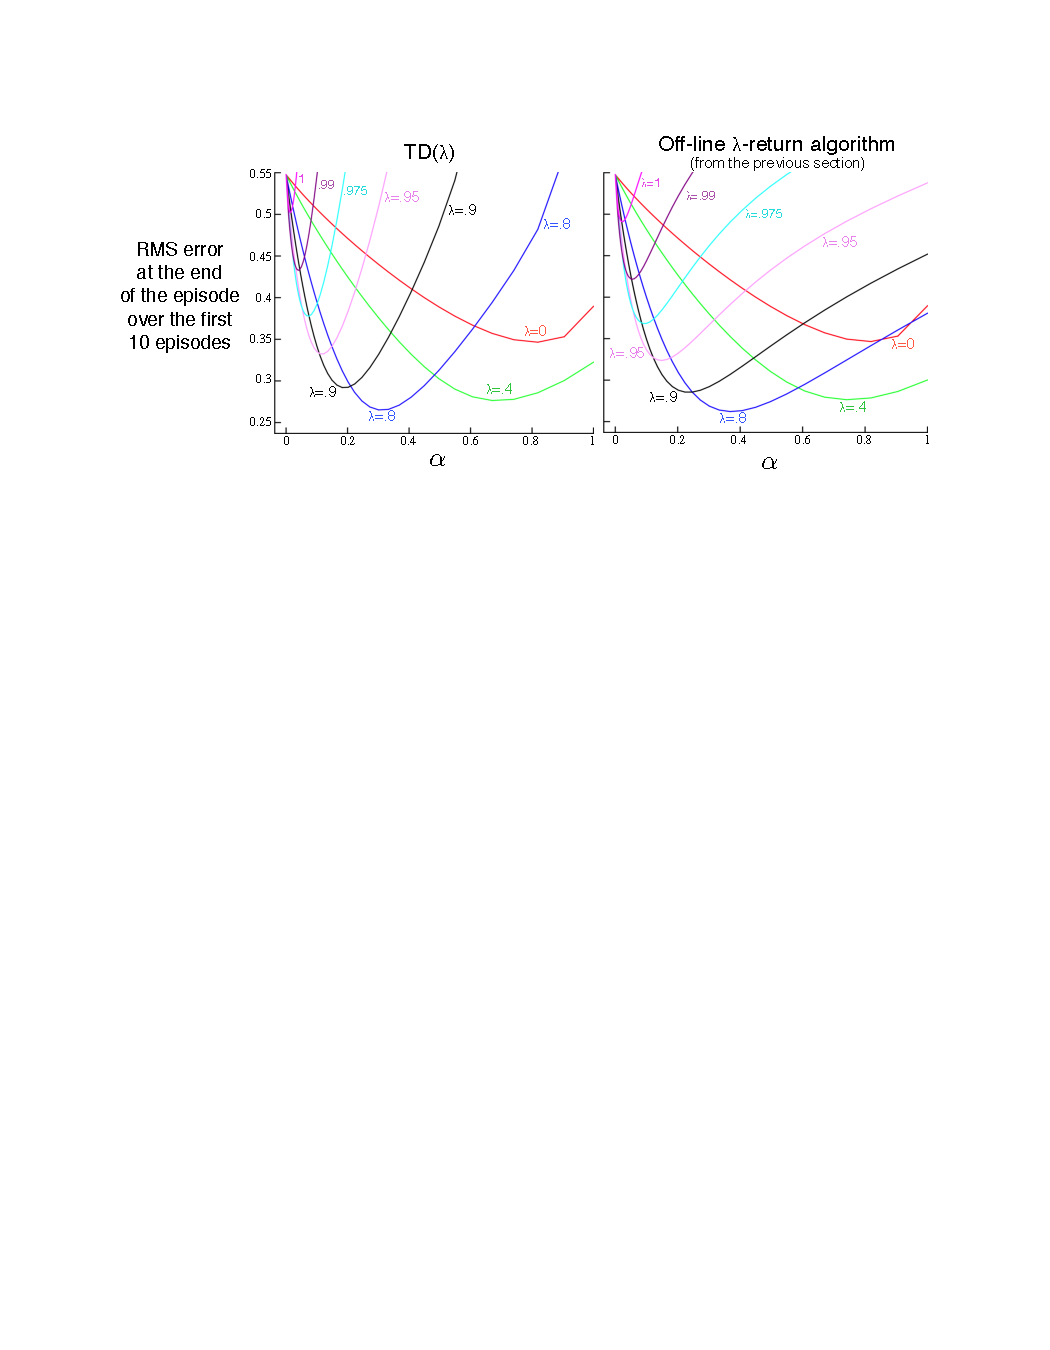
\includegraphics[height=5cm]{fig/lec11/TD_lambda_vs_offline_lambda.pdf}
\caption{Prediction accuracy comparison based on 19-state random walk example from \figref{fig:Random_Walk_19_States} (source: R. Sutton and G. Barto, Reinforcement learning: an introduction, 2018, \href{https://creativecommons.org/licenses/by-nc-nd/2.0/}{CC BY-NC-ND 2.0})}
\label{fig:TD_lambda_vs_offline_lambda}
\end{figure}
}

%%%%%%%%%%%%%%%%%%%%%%%%%%%%%%%%%%%%%%%%%%%%%%%%%%%%%%%%%%%%%%%%%%
\section{Online \texorpdfstring{$\lambda$}{Lambda}-Return Updates} 
%%%%%%%%%%%%%%%%%%%%%%%%%%%%%%%%%%%%%%%%%%%%%%%%%%%%%%%%%%%%%%%%%%
\begin{frame}
\frametitle{Table of Contents}
\tableofcontents[currentsection]
\end{frame}

%%%%%%%%%%%%%%%%%%%%%%%%%%%%%%%%%%%%%%%%%%%%%%%%%%%%%%%%%%%%%
%% Truncated $\lambda$-Returns for Online Updates %%
%%%%%%%%%%%%%%%%%%%%%%%%%%%%%%%%%%%%%%%%%%%%%%%%%%%%%%%%%%%%%
\frame{\frametitle{Truncated $\lambda$-Returns for Online Updates}
\begin{itemize}
	\item Recall the truncated $\lambda$-return after $h$ steps 
	\begin{equation*}
		g_{k:h}^\lambda = (1-\lambda)\sum_{n=1}^{h-k-1}\lambda^{(n-1)}g_{k:k+n} + \lambda^{h-k-1}g_{k:h}\,.
	\end{equation*}\pause
	\item If $h<T$ then we can perform online updates since $\bm{w}$ is changed within an episode.\pause
	\item Implementation is very similar to $n$-step bootstrapping, also forward view (e.g., still delayed with increased memory demand):  
\end{itemize}
\begin{equation*}
\begin{split}
	 \delta_k'&= r_{k+1} + \gamma \hat{v}(\bm{x}_{k+1}, \bm{w}_k) - \hat{v}(\bm{x}_{k}, \bm{w}_k),\\
	 g_{k:k+n}^\lambda &= \hat{v}(\bm{x}_{k}, \bm{w}_{k-1}) + \sum_{i=k}^{k+n-1}(\gamma\lambda)^{i-k}\delta_i',\\
	 \bm{w}_{k+n} &= \bm{w}_{k+n-1} + \alpha\left[g_{k:k+n}^\lambda - \hat{v}(\bm{x}_k, \bm{w}_{k+n-1})\right]\nabla_{\bm{w}}\hat{v}(\bm{x}_k, \bm{w}_{k+n-1}) .
\end{split}	
\end{equation*}
}

%%%%%%%%%%%%%%%%%%%%%%%%%%%%%%%%%%%%%%%%%%%%%%%%%%%%%%%%%%%%%
%% Increase Approximation Quality by Redoing Updates (1)%%
%%%%%%%%%%%%%%%%%%%%%%%%%%%%%%%%%%%%%%%%%%%%%%%%%%%%%%%%%%%%%
\frame{\frametitle{Increase Approximation Quality by Redoing Updates (1)}
General trade-off regarding the truncated $\lambda$-returns (forward view):
\begin{itemize}
	\item If $n$ is small: delay and memory demand are low.
	\item If $n$ is high: approximation of offline $\lambda$-returns is more accurate.
\end{itemize}\pause
Idea to solve this compromise: \hl{redoing updates}.
\begin{itemize}
	\item If new data is available, we go back and redo all previous updates.
	\item Reuse data samples $\bm{\mathcal{D}}_k\sim\left\langle \bm{x}_k, r_k, \bm{x}_{k+1}\right\rangle$.\pause 
	\item Update parameter vector $\bm{w}_k^h$ at $k$-th time step up to horizon $h$.
\end{itemize}
\begin{figure}
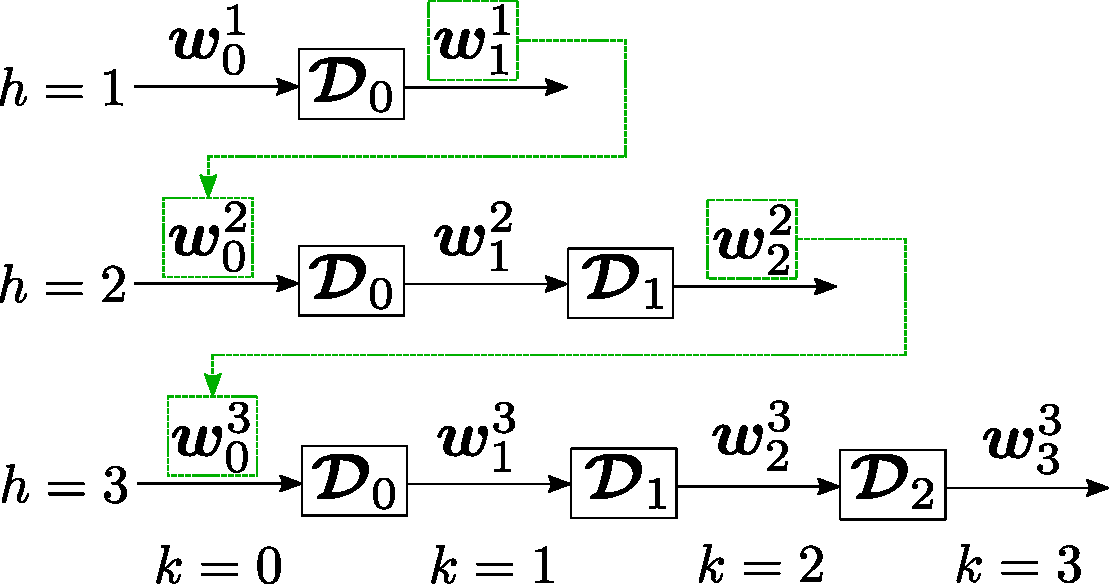
\includegraphics[height=3.5cm]{fig/lec11/Redoing_Updates.pdf}
\caption{Simplified flowchart for redoing updates at time step $k$ and horizon $h$}
\label{fig:Redoing_Updates}
\end{figure}
}

%%%%%%%%%%%%%%%%%%%%%%%%%%%%%%%%%%%%%%%%%%%%%%%%%%%%%%%%%%%%%
%% Increase Approximation Quality by Redoing Updates (2)%%
%%%%%%%%%%%%%%%%%%%%%%%%%%%%%%%%%%%%%%%%%%%%%%%%%%%%%%%%%%%%%
\frame{\frametitle{Increase Approximation Quality by Redoing Updates (2)}
The update sequence from example \figref{fig:Redoing_Updates} using semi-gradients:
\begin{alignat*}{2}
&h=1: \quad &&\bm{w}_1^1 = \bm{w}_0^1 + \alpha\left[g_{0:1}^\lambda - \hat{v}(\bm{x}_0, \bm{w}_0^1)\right]\nabla_{\bm{w}} \hat{v}(\bm{x}_0, \bm{w}_0^1)\\
\\
&h=2: \quad &&\bm{w}_1^2 = \bm{w}_0^2 + \alpha\left[g_{0:2}^\lambda - \hat{v}(\bm{x}_0, \bm{w}_0^2)\right]\nabla_{\bm{w}} \hat{v}(\bm{x}_0, \bm{w}_0^2)\\
&						&&\bm{w}_2^2 = \bm{w}_1^2 + \alpha\left[g_{1:2}^\lambda - \hat{v}(\bm{x}_1, \bm{w}_1^2)\right]\nabla_{\bm{w}} \hat{v}(\bm{x}_1, \bm{w}_1^2)\\ 
\\
&h=3: \quad &&\bm{w}_1^3 = \bm{w}_0^3 + \alpha\left[g_{0:3}^\lambda - \hat{v}(\bm{x}_0, \bm{w}_0^3)\right]\nabla_{\bm{w}} \hat{v}(\bm{x}_0, \bm{w}_0^3)\\
&						&&\bm{w}_2^3 = \bm{w}_1^3 + \alpha\left[g_{1:3}^\lambda - \hat{v}(\bm{x}_1, \bm{w}_1^3)\right]\nabla_{\bm{w}} \hat{v}(\bm{x}_1, \bm{w}_1^3)\\
&						&&\bm{w}_3^3 = \bm{w}_2^3 + \alpha\left[g_{2:3}^\lambda - \hat{v}(\bm{x}_2, \bm{w}_2^3)\right]\nabla_{\bm{w}} \hat{v}(\bm{x}_2, \bm{w}_2^3)  
\end{alignat*}
}

%%%%%%%%%%%%%%%%%%%%%%%%%%%%%%%%%%%%%%%%%%%%%%%%%%%%%%%%%%%%%
%% Increase Approximation Quality by Redoing Updates (3)%%
%%%%%%%%%%%%%%%%%%%%%%%%%%%%%%%%%%%%%%%%%%%%%%%%%%%%%%%%%%%%%
\frame{\frametitle{Increase Approximation Quality by Redoing Updates (3)}
Generalization of the example:
\begin{block}{Online $\lambda$-return}
Having samples $\bm{\mathcal{D}}_k\sim\left\langle \bm{x}_k, r_k, \bm{x}_{k+1}\right\rangle$ up to horizon $h$ available, the general online $\lambda$-return update is
\begin{equation}
	\bm{w}_{k+1}^h = \bm{w}_k^h + \alpha\left[g_{k:h}^\lambda - \hat{v}(\bm{x}_k, \bm{w}_k^h)\right]\nabla_{\bm{w}} \hat{v}(\bm{x}_k, \bm{w}_k^h), \,\,\,\, 0 \leq k \leq h \leq T
	\label{eq:online_lambda_return_update}
\end{equation}
with the final parameter vector $\bm{w}_k=\bm{w}_{k}^k$ at the given time step.
\end{block}
\pause
\begin{itemize}
	\item Online approach: a new $\bm{w}_k$ is calculated at each step using only information available at step $k$.\pause
	\item Obviously, the approach is very computationally demanding.
	\begin{itemize}
		\item Computations increase with every time step.
		\item Is likely to become infeasible for long episodes.
	\end{itemize}
\end{itemize}
}

%%%%%%%%%%%%%%%%%%%%%%%%%%%%%%%%%%%%%%%%%%%%%%%%%%%%%%%%%%%%%
%% Comparison Online Vs. Offline $\lambda$-Returns %%
%%%%%%%%%%%%%%%%%%%%%%%%%%%%%%%%%%%%%%%%%%%%%%%%%%%%%%%%%%%%%
\frame{\frametitle{Comparison Online Vs. Offline $\lambda$-Returns}
\begin{itemize}
	\item Through the repeated updates, the online $\lambda$-return algorithm can even increase the prediction quality compared to its offline variant.
\end{itemize}
\vspace{0.3cm}
\begin{figure}
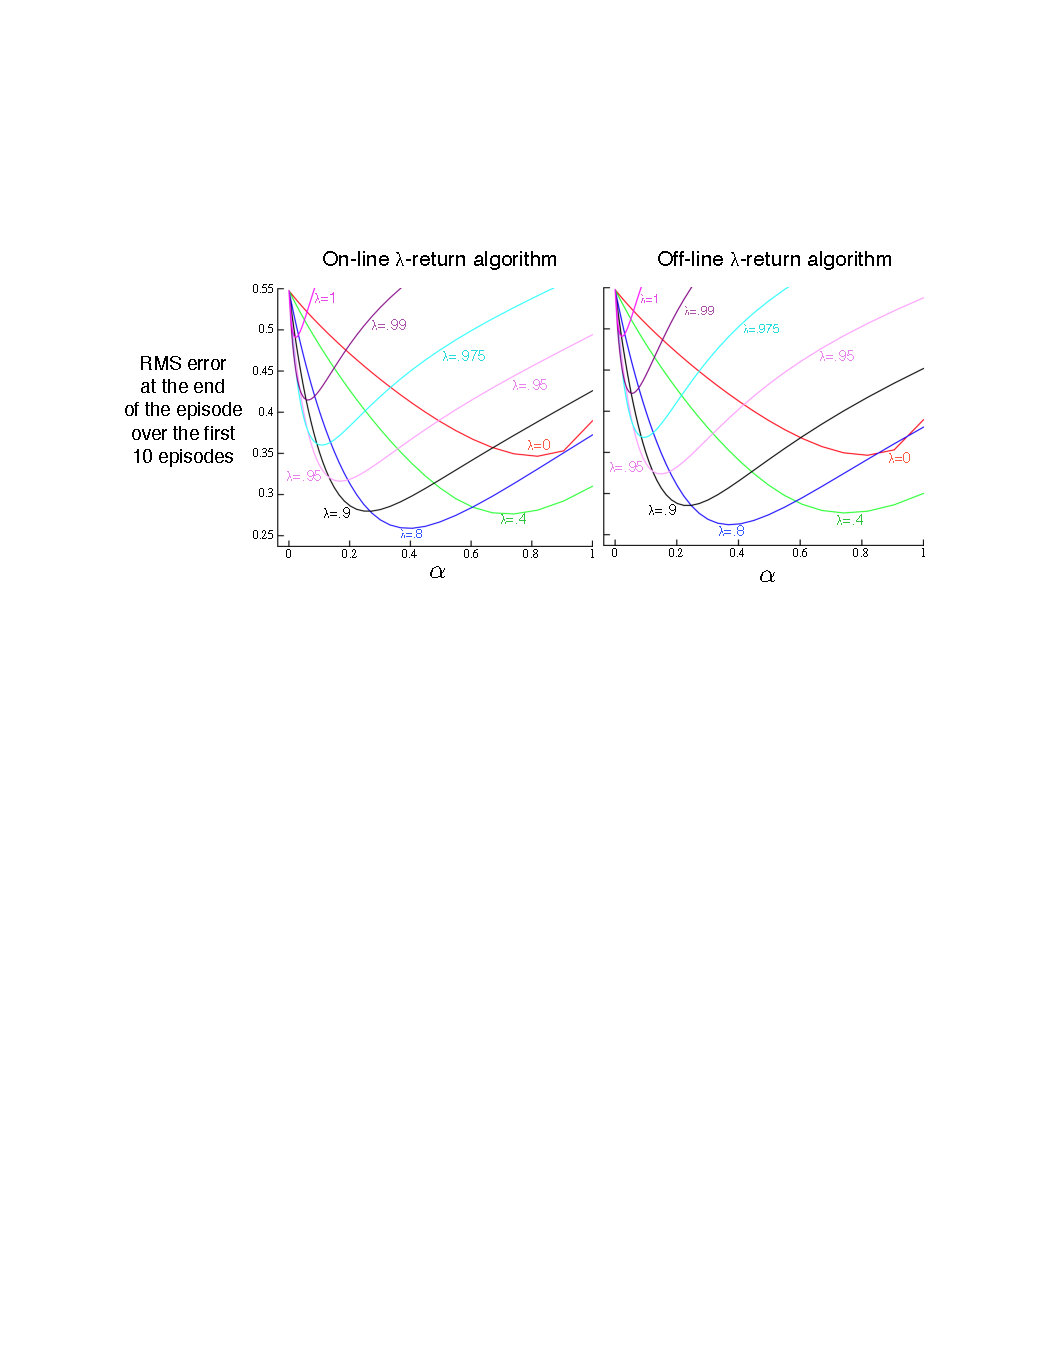
\includegraphics[height=4.75cm]{fig/lec11/Offline_Online_Lambda_Returns.pdf}
\caption{Prediction accuracy comparison based on 19-state random walk example from \figref{fig:Random_Walk_19_States} (source: R. Sutton and G. Barto, Reinforcement learning: an introduction, 2018, \href{https://creativecommons.org/licenses/by-nc-nd/2.0/}{CC BY-NC-ND 2.0})}
\label{fig:Offline_Online_Lambda_Returns}
\end{figure}
}


%%%%%%%%%%%%%%%%%%%%%%%%%%%%%%%%%%%%%%%%%%%%%%%%%%%%%%%%%%%%%
%% True Online TD(\$\lambda$) for Linear Approximation %%
%%%%%%%%%%%%%%%%%%%%%%%%%%%%%%%%%%%%%%%%%%%%%%%%%%%%%%%%%%%%%
\frame{\frametitle{True Online TD($\lambda$) for Linear Approximation}
If linear function approximation $\hat{v}=\tilde{\bm{x}}\T\bm{w}$ is applied the
\begin{itemize}
	\item online $\lambda$-return updates \eqref{eq:online_lambda_return_update} and 
	\item the elegant implementation using eligibility traces \eqref{eq:Elig_trace}
\end{itemize}
can be nicely combined. \pause By doing so we receive
\begin{itemize}
	\item backward-viewing linear algorithm which
	\item is denoted as \hl{'true' online TD($\lambda$)} because it is not an approximation of the offline $\lambda$-returns as the regular TD($\lambda$) from \algoref{algo:Semi_gradient_TD_lambda}.
\end{itemize}\pause
The true online TD($\lambda$) update equations are\footnote[1]{\onslide<3->{Find derivation and more information: H. van Seijen et al., \textit{True Online Temporal-Difference Learning}, Journal of Machine Learning Research, Vol. 17, 2016}}:
\begin{equation}
	\begin{split}
	  \bm{z}_k &= \gamma\lambda\bm{z}_{k-1} + (1-\alpha\gamma\lambda\tilde{\bm{x}}\T_k\bm{z}_{k-1})\tilde{\bm{x}}_k,\\
		\delta_k &=r_{k+1} + \gamma\tilde{\bm{x}}\T_{k+1}\bm{w}_k  -\tilde{\bm{x}}\T_{k}\bm{w}_k,\\
		\bm{w}_{k+1} &= \bm{w}_k + \alpha\delta_k\bm{z}_k+\alpha\left(\tilde{\bm{x}}\T_k\bm{w}_k - \tilde{\bm{x}}\T_k\bm{w}_{k-1}\right)\left(\bm{z}_k - \tilde{\bm{x}}_k\right).
	\end{split}
\end{equation}
}

%%%%%%%%%%%%%%%%%%%%%%%%%%%%%%%%%%%%%%%%%%%%%%%%%%%%%%%%%%%%%
%% Algorithmic Implementation: True Online TD($\lambda$) %%
%%%%%%%%%%%%%%%%%%%%%%%%%%%%%%%%%%%%%%%%%%%%%%%%%%%%%%%%%%%%%
\frame{\frametitle{Algorithmic Implementation: True Online TD($\lambda$)}
\setlength{\algomargin}{0.5em}
\begin{algorithm}[H]
\small
\SetKwInput{Input}{input} 
\SetKwInput{Output}{output}
\SetKwInput{Init}{init}
\SetKwInput{Param}{parameter}
\Input{a policy $\pi$ to be evaluated}
\Input{a feature representation $\tilde{\bm{x}}$ with $\tilde{\bm{x}}_T=0$ (i.e., $\hat{v}(\tilde{\bm{x}}_T,\cdot)=0$)}
\Param{step size $\alpha\in\left\{\mathbb{R}|0<\alpha<1\right\}$, decay rate $\lambda\in\left\{\mathbb{R}|0 \leq \lambda \leq 1\right\}$}
\Init{value-function weights $\bm{w}\in\mathbb{R}^\zeta$ arbitrarily}
 \For{$j=1,2,\ldots$ episodes}{
		initialize $\bm{x}_{0}$\;
		set $\bm{z}=0$ and $\hat{v}_{old}=0$\;
		\For{$k=0, 1, 2 \ldots $ time steps}{
			$u_k \leftarrow$ apply action from $\pi(\bm{x}_k)$\;
			observe $\bm{x}_{k+1}$ and $r_{k+1}$\;
			$\hat{v}\leftarrow\tilde{\bm{x}}\T_k\bm{w}$\;
			$\hat{v}'\leftarrow\tilde{\bm{x}}\T_{k+1}\bm{w}$\;
			$\delta\leftarrow r_{k+1}+\gamma\hat{v}'-\hat{v}$\;
			$\bm{z}\leftarrow \gamma\lambda\bm{z} + (1-\alpha\gamma\lambda\tilde{\bm{x}}\T_k\bm{z})\tilde{\bm{x}}_k$\;
			$\bm{w} \leftarrow \bm{w} + \alpha(\delta +\hat{v} - \hat{v}_{old})\bm{z} - \alpha(\hat{v} - \hat{v}_{old})\tilde{\bm{x}}_k$\; 
			$\hat{v}_{old}\leftarrow\hat{v}'$\;
			exit loop if $\bm{x}_{k+1}$ is terminal\;
		}
	}
\caption{True Online TD($\lambda$) (output: parameter vector $\bm{w}$ for $\hat{v}_\pi$)}
\label{algo:True_Online_TD_Lambda}
\end{algorithm}
}

%%%%%%%%%%%%%%%%%%%%%%%%%%%%%%%%%%%%%%%%%%%%%%%%%%%%%%%%%%%%%%%%%%
\section{Sarsa(\texorpdfstring{$\lambda$}{Lambda})} 
%%%%%%%%%%%%%%%%%%%%%%%%%%%%%%%%%%%%%%%%%%%%%%%%%%%%%%%%%%%%%%%%%%
\begin{frame}
\frametitle{Table of Contents}
\tableofcontents[currentsection]
\end{frame}

%%%%%%%%%%%%%%%%%%%%%%%%%%%%%%%%%%%%%%%%%%%%%%%%%%%%%%%%%%%%%
%% Transfer for Action Values %%
%%%%%%%%%%%%%%%%%%%%%%%%%%%%%%%%%%%%%%%%%%%%%%%%%%%%%%%%%%%%%
\frame{\frametitle{Transfer for Action Values}
First, transfer truncated $\lambda$-returns to action values (forward view):
\begin{equation}
\begin{split}
		g_{k:h}^\lambda &= (1-\lambda)\sum_{n=1}^{h-k-1}\lambda^{(n-1)}g_{k:k+n} + \lambda^{h-k-1}g_{k:h},\\
		g_{k:k+n} &= r_{k+1}+\gamma r_{k+2}+\cdots+\gamma^{n-1} r_{k+n}+\gamma^n\hat{q}(\bm{x}_{k+n}, u_{k+n}, \bm{w}_{k+n-1}).
\end{split}	
\end{equation}\pause
From that, the forward view \hl{offline $\lambda$-return} update for $\hat{q}$ is:
\begin{equation}
	\bm{w}_{k+1} = \bm{w}_k+\alpha\left[g_k^\lambda - \hat{q}(\bm{x}_k, u_k, \bm{w}_k)\right]\nabla_{\bm{w}}\hat{q}(\bm{x}_k, u_k\bm{w}_k) .
	\label{eq:offline_lambda_return_action}
\end{equation}\pause
The backward view approximation known as \hl{Sarsa($\lambda$)} is then:
\begin{equation}
\begin{split}
		\delta_k &=r_{k+1} + \gamma \hat{q}(\bm{x}_{k+1}, u_{k+1}, \bm{w}_k) -\hat{q}(\bm{x}_{k}, u_{k}, \bm{w}_k),\\
		\bm{z}_k &=\gamma\lambda\bm{z}_{k-1}+\nabla_{\bm{w}}\hat{q}(\bm{x}_k, u_k, \bm{w}_k),\quad \bm{z}_{0}=0,\\
		 \bm{w}_{k+1} &=  \bm{w}_k + \alpha\delta_k\bm{z}_k .
\end{split}	
\end{equation}
}

%%%%%%%%%%%%%%%%%%%%%%%%%%%%%%%%%%%%%%%%%%%%%%%%%%%%%%%%%%%%%
%% Semi-Gradient Sarsa %%
%%%%%%%%%%%%%%%%%%%%%%%%%%%%%%%%%%%%%%%%%%%%%%%%%%%%%%%%%%%%%
\frame{\frametitle{Algorithmic Implementation: Semi-Gradient Sarsa($\lambda$)}
\setlength{\algomargin}{0.5em}
\begin{algorithm}[H]
\small
\SetKwInput{Input}{input} 
\SetKwInput{Output}{output}
\SetKwInput{Init}{init}
\SetKwInput{Param}{parameter}
\Input{a differentiable function $\hat{q}:\mathbb{R}^\kappa\times\mathbb{R}^\zeta\rightarrow\mathbb{R}$}
\Input{a policy $\pi$ (only if estimating $q_\pi$)}
\Param{$\alpha\in\left\{\mathbb{R}|0<\alpha<1\right\}$, $\varepsilon\in\left\{\mathbb{R}|0<\varepsilon<<1\right\}$, $\lambda\in\left\{\mathbb{R}|0 \leq \lambda \leq 1\right\}$}
\Init{parameter vector $\bm{w}\in\mathbb{R}^\zeta$ arbitrarily}
 \For{$j=1,2,\ldots$ episodes}{
		initialize $\bm{x}_{0}$ and set $\bm{z}=0$\;
		$u_0 \leftarrow$ choose action from $\pi(\bm{x}_0)$ or $\varepsilon$-greedy on $\hat{q}(\bm{x}_0, \cdot, \bm{w})$\;
		\For{$k=0, 1, 2 \ldots $ time steps}{
			apply action $u_k$, observe $\bm{x}_{k+1}$ and $r_{k+1}$\;
			\lIf{$\bm{x}_{k+1}$ is terminal}{$\delta\leftarrow r_{k+1} - \hat{q}(\bm{x}_k, u_k, \bm{w})$}
			\Else{
				$u_{k+1}\leftarrow \pi(\bm{x}_{k+1})$ or $\varepsilon$-greedy on $\hat{q}(\bm{x}_{k+1},\cdot, \bm{w})$\;
				$\delta\leftarrow r_{k+1} +\gamma \hat{q}(\bm{x}_{k+1}, u_{k+1}, \bm{w}) - \hat{q}(\bm{x}_k, u_k, \bm{w})$\;
			}
			$\bm{z}\leftarrow \gamma\lambda\bm{z}+\nabla_{\bm{w}}\hat{q}(\bm{x}_k, u_k, \bm{w})$\;
			$\bm{w} \leftarrow \bm{w} + \alpha\delta\bm{z}$\; 
			exit loop if $\bm{x}_{k+1}$ is terminal\; 
		}
	}
\caption{Semi-gradient Sarsa($\lambda$) (output: parameter vector $\bm{w}$ for $\hat{q}_\pi$ or $\hat{q}^*$)}
\label{algo:Semi_gradient_Sarsa_Lambda}
\end{algorithm}
}

%%%%%%%%%%%%%%%%%%%%%%%%%%%%%%%%%%%%%%%%%%%%%%%%%%%%%%%%%%%%%
%% Sarsa Learning Comparison in Gridworld Example %%
%%%%%%%%%%%%%%%%%%%%%%%%%%%%%%%%%%%%%%%%%%%%%%%%%%%%%%%%%%%%%
\frame{\frametitle{Sarsa Learning Comparison in Gridworld Example}
\begin{itemize}
	\item $\lambda$ can be interpreted as the discounting factor acting on the eligibility trace (see right-most panel below).
	\item Intuitive interpretation: more recent transitions are more certain/relevant for the current update step. 
\end{itemize}
\vspace{0.3cm}
\begin{figure}
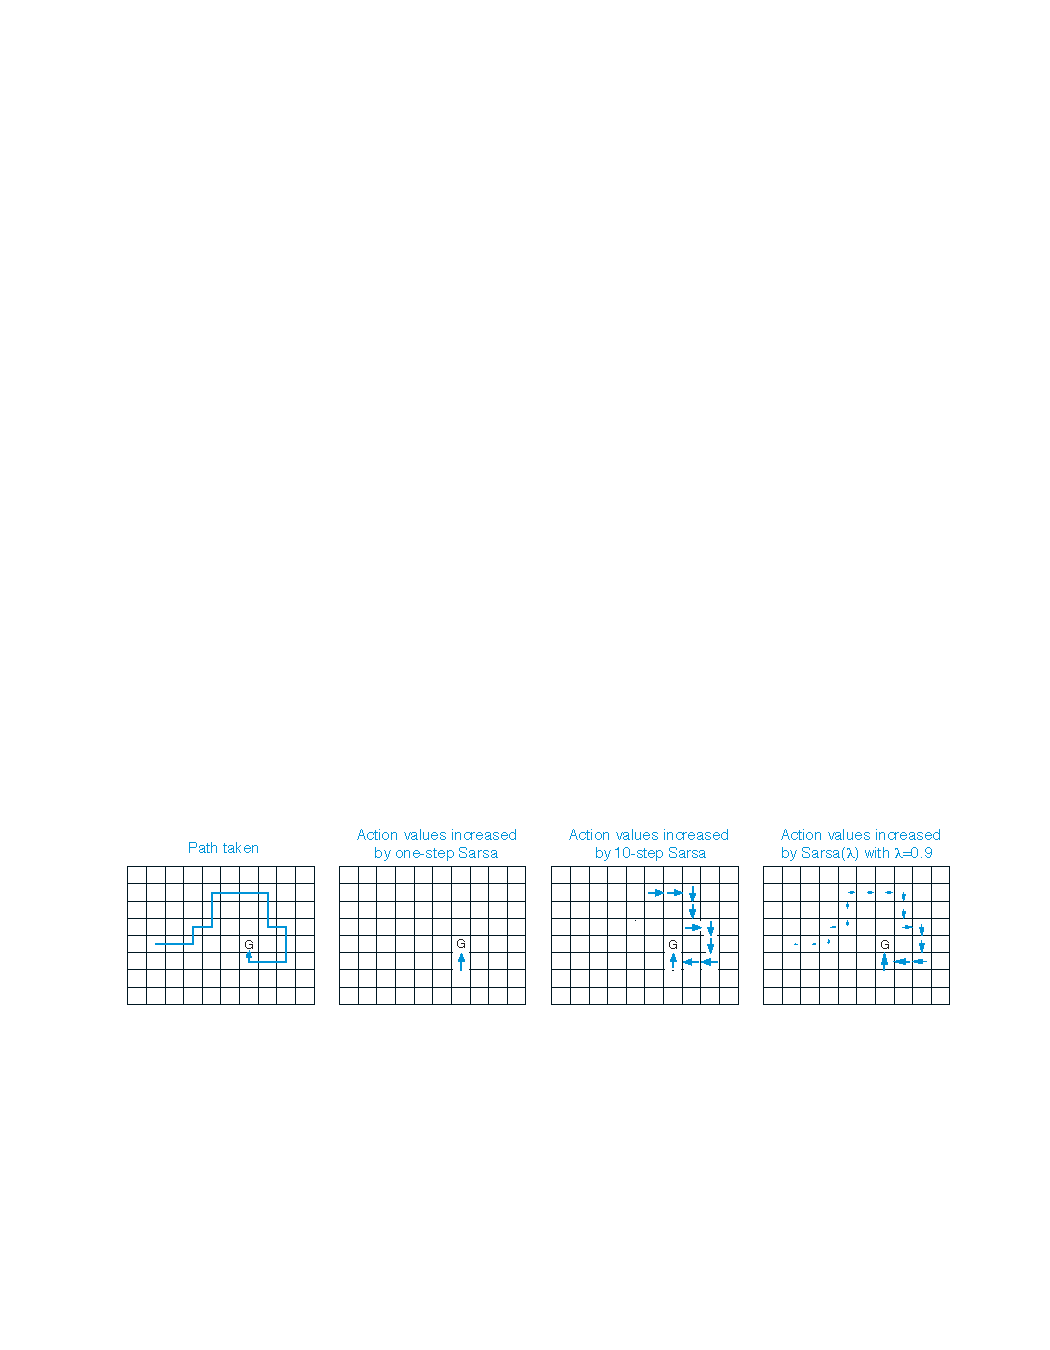
\includegraphics[width=12cm]{fig/lec11/Traces_Sarsa_Gridworld.pdf}
\caption{Sarsa variants after an arbitrary episode within a gridworld environment -- arrows indicate action-value change starting from initially zero estimates (source: R. Sutton and G. Barto, Reinforcement learning: an introduction, 2018, \href{https://creativecommons.org/licenses/by-nc-nd/2.0/}{CC BY-NC-ND 2.0})}
\label{fig:Traces_Sarsa_Gridworld}
\end{figure}
}

%%%%%%%%%%%%%%%%%%%%%%%%%%%%%%%%%%%%%%%%%%%%%%%%%%%%%%%%%%%%%
%% Sarsa($\lambda$) vs $n$-step Sarsa on Mountain Car Task %%
%%%%%%%%%%%%%%%%%%%%%%%%%%%%%%%%%%%%%%%%%%%%%%%%%%%%%%%%%%%%%
\frame{\frametitle{Sarsa($\lambda$) vs $n$-Step Sarsa on Mountain Car Task}
\begin{itemize}
	\item Sarsa($\lambda$) is able to learn significantly faster than any $n$-step variant.
	\item However, only intermediate performance is shown after 50 episodes.
\end{itemize}
\vspace{0.3cm}
\begin{figure}
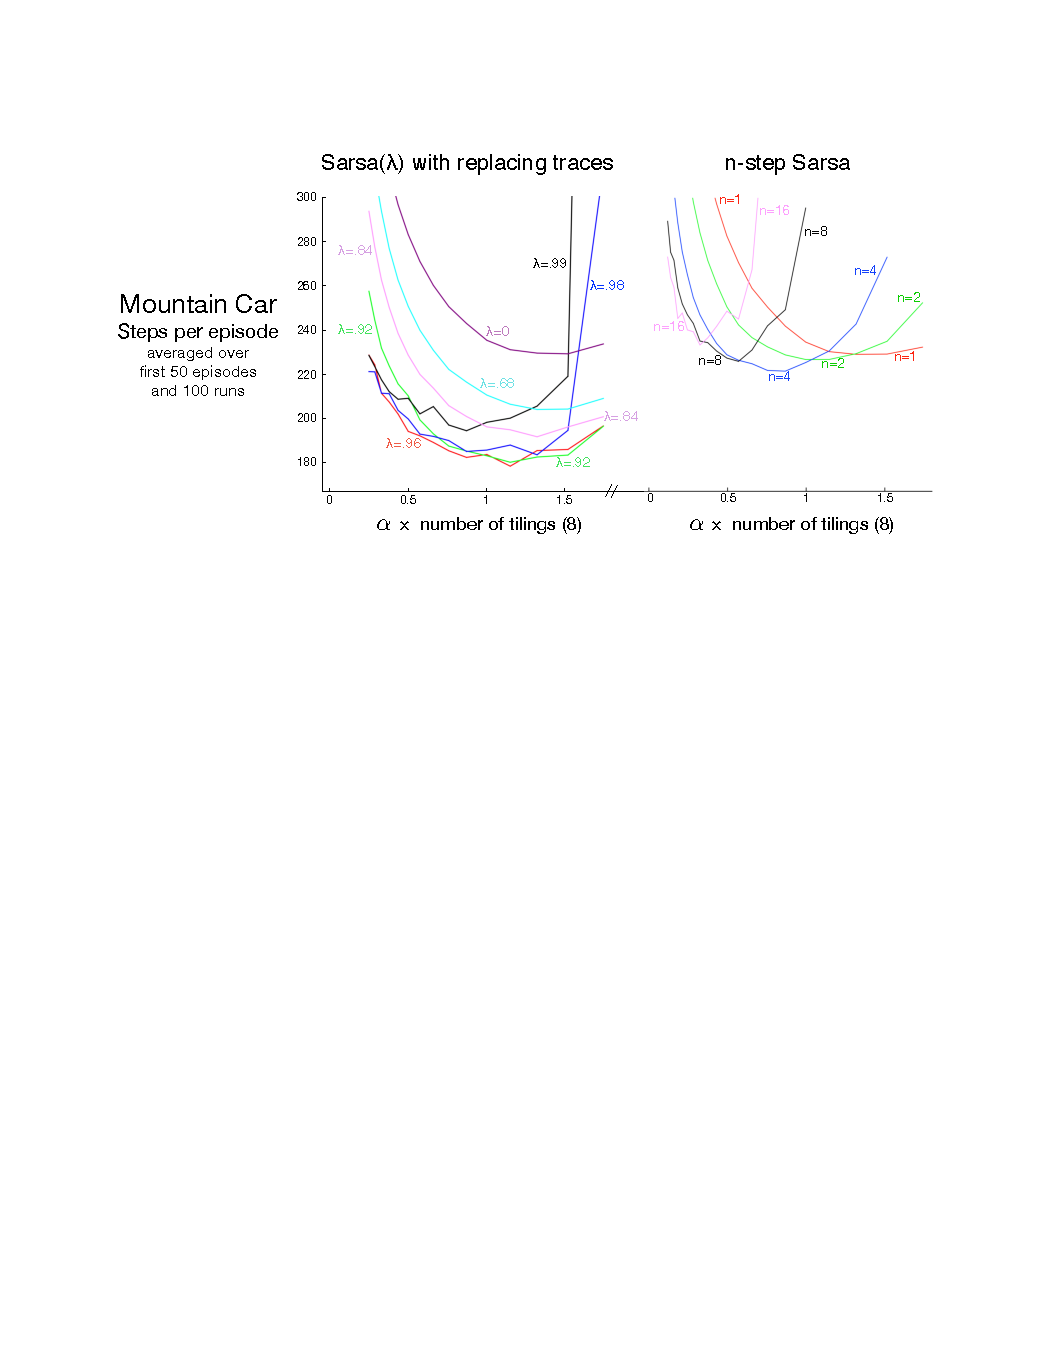
\includegraphics[width=10cm]{fig/lec11/Sarsa_Lambda_Mountain_Car.pdf}
\caption{Sarsa-based control performance comparison based on previous example from \figref{fig:Mountain_car_gym}. Both algorithms use linear function approximation and tile coding (source: R. Sutton and G. Barto, Reinforcement learning: an introduction, 2018, \href{https://creativecommons.org/licenses/by-nc-nd/2.0/}{CC BY-NC-ND 2.0})}
\label{fig:Sarsa_Lambda_Mountain_Car}
\end{figure}
}

%%%%%%%%%%%%%%%%%%%%%%%%%%%%%%%%%%%%%%%%%%%%%%%%%%%%%%%%%%%%%
%% True Online Sarsa($\lambda$) %%
%%%%%%%%%%%%%%%%%%%%%%%%%%%%%%%%%%%%%%%%%%%%%%%%%%%%%%%%%%%%%
\frame{\frametitle{True Online Sarsa($\lambda$)}
\begin{itemize}
	\item Likewise TD($\lambda$) for state values, Sarsa($\lambda$) is not an exact backward view implementation of the offline $\lambda$-return algorithm \eqref{eq:offline_lambda_return_action}.\pause
 \item To improve the Sarsa($\lambda$) performance we again have two options:
\begin{itemize}
	\item Redoing updates: Online Sarsa($\lambda$) (e.g., with non-linear function approximation, direct transfer from \eqref{eq:online_lambda_return_update}),
	\item or re-use the true online implementation with linear approximators for action values.
\end{itemize}
\end{itemize}\pause
\vspace{0.5cm}
\begin{itemize}
	\item The true online Sarsa($\lambda$) updates are analog to TD($\lambda$), but the features additionally contain action information $\tilde{\bm{x}}=\bm{f}(\bm{x},u)$ :
\end{itemize}
\begin{equation}
	\begin{split}
	  \bm{z}_k &= \gamma\lambda\bm{z}_{k-1} + (1-\alpha\gamma\lambda\tilde{\bm{x}}\T_k\bm{z}_{k-1})\tilde{\bm{x}}_k,\\
		\delta_k &=r_{k+1} + \gamma\tilde{\bm{x}}\T_{k+1}\bm{w}_k  -\tilde{\bm{x}}\T_{k}\bm{w}_k,\\
		\bm{w}_{k+1} &= \bm{w}_k + \alpha\delta_k\bm{z}_k+\alpha\left(\tilde{\bm{x}}\T_k\bm{w}_k - \tilde{\bm{x}}\T_k\bm{w}_{k-1}\right)\left(\bm{z}_k - \tilde{\bm{x}}_k\right).
	\end{split}
\end{equation}
}

%%%%%%%%%%%%%%%%%%%%%%%%%%%%%%%%%%%%%%%%%%%%%%%%%%%%%%%%%%%%%
%% Algorithmic Implementation: True Online Sarsa($\lambda$) %%
%%%%%%%%%%%%%%%%%%%%%%%%%%%%%%%%%%%%%%%%%%%%%%%%%%%%%%%%%%%%%
\frame{\frametitle{Algorithmic Implementation: True Online Sarsa($\lambda$)}
\setlength{\algomargin}{0.5em}
\begin{algorithm}[H]
\small
\SetKwInput{Input}{input} 
\SetKwInput{Output}{output}
\SetKwInput{Init}{init}
\SetKwInput{Param}{parameter}
\Input{a policy $\pi$ to be evaluated}
\Input{a feature representation $\tilde{\bm{x}}$ with $\tilde{\bm{x}}_T=0$ (i.e., $\hat{q}(\tilde{\bm{x}}_T,\cdot,\cdot)=0$)}
\Param{$\alpha\in\left\{\mathbb{R}|0<\alpha<1\right\}$, $\varepsilon\in\left\{\mathbb{R}|0<\varepsilon<<1\right\}$, $\lambda\in\left\{\mathbb{R}|0 \leq \lambda \leq 1\right\}$}
\Init{value-function weights $\bm{w}\in\mathbb{R}^\zeta$ arbitrarily}
 \For{$j=1,2,\ldots$ episodes}{
		initialize $\bm{x}_{0}$	and set	$u_0 \leftarrow$ from $\pi(\bm{x}_0)$ or $\varepsilon$-greedy on $\hat{q}(\bm{x}_0, \cdot, \bm{w})$\;
		set $\bm{z}=0$ and $\hat{q}_{old}=0$\;
		\For{$k=0, 1, 2 \ldots $ time steps}{
			apply action $u_k$, observe $\bm{x}_{k+1}$ and $r_{k+1}$\;
			$u_{k+1} \leftarrow$ choose action from $\pi(\bm{x}_{k+1})$ or $\varepsilon$-greedy on $\hat{q}(\bm{x}_{k+1}, \cdot, \bm{w})$\;
			$\hat{q}\leftarrow\tilde{\bm{x}}\T_k\bm{w}$ and $\hat{q}'\leftarrow\tilde{\bm{x}}\T_{k+1}\bm{w}$\;
			$\delta\leftarrow r_{k+1}+\gamma\hat{q}'-\hat{q}$\;
			$\bm{z}\leftarrow \gamma\lambda\bm{z} + (1-\alpha\gamma\lambda\tilde{\bm{x}}\T_k\bm{z})\tilde{\bm{x}}_k$\;
			$\bm{w} \leftarrow \bm{w} + \alpha(\delta +\hat{q} - \hat{q}_{old})\bm{z} - \alpha(\hat{q} - \hat{q}_{old})\tilde{\bm{x}}_k$\; 
			$\hat{q}_{old}\leftarrow\hat{q}'$\;
			exit loop if $\bm{x}_{k+1}$ is terminal\;
		}
	}
\caption{True Online Sarsa($\lambda$) (output: parameter vector $\bm{w}$ for $\hat{q}_\pi$ or $\hat{q}^*$)}
\label{algo:True_Online_TD_Sarsa}
\end{algorithm}
}

%%%%%%%%%%%%%%%%%%%%%%%%%%%%%%%%%%%%%%%%%%%%%%%%%%%%%%%%%%%%%
%% Summary %%
%%%%%%%%%%%%%%%%%%%%%%%%%%%%%%%%%%%%%%%%%%%%%%%%%%%%%%%%%%%%%
\begin{frame}
\frametitle{Summary: What You've Learned Today}
\begin{itemize}
	\item Multiple $n$-step return estimates can be weighted to form a compound update (adds more degrees of freedom).\pause
	\item $\lambda$-returns use this idea with exponentially-decaying weights.
	\begin{itemize}
		\item However, like $n$-step bootstrapping also $\lambda$-returns are forward-viewing and, therefore suffer from increased memory demand and delay times.
	\end{itemize}\pause
	\item Using eligibility traces we introduce backward-facing algorithms:
		\begin{itemize}
			\item The trace is acting as a short-term memory.
			\item How important was a parameter for the current value update? 
		\end{itemize}\pause
	\item TD$(\lambda)$	is using the traces for state-value prediction.
	\begin{itemize}
		\item Applicable with general nonlinear function approximation.
		\item However, not an exact representation of $\lambda$-returns.
	\end{itemize}\pause
	\item Only if linear function approximation is used, true online TD$(\lambda)$ allows identically backward-facing updates as $\lambda$-returns. \pause
	\item Transfer to action values by Sarsa is straightforward.
\end{itemize}
\end{frame}